\documentclass{article}
\usepackage{amsmath}
\usepackage{tikz,pgfplots}
\usepackage[margin=1in]{geometry}
\begin{document}
\title{Answer to Assignment 6}
\author{Phumin Walaipatchara}
\date{}
\maketitle
\noindent\textbf{Question 1}
\\\\
\indent First, find the eigenvectors and eigenvalues of $A$
\\\\
$
\indent\indent(.4 - \lambda)(1.2 - \lambda) - (.4 \times -.3) = 0 
\\\\
\indent\indent .48 - .4\lambda - 1.2\lambda + \lambda^2 + .12 = 0
\\\\
\indent\indent \lambda^2 - 1.6\lambda + .6 = 0
\\\\
\indent\indent (\lambda - .6) \times (\lambda  - 1) = 0
\\\\
\indent\indent \lambda = .6$ and $1$
\\\\\\\\
\indent Second, find the eigenvectors of $A$
$
\\\\
\indent\indent\lambda = .6
\\\\
\indent\indent\begin{bmatrix}-.2&-.3\\.4&.6\end{bmatrix}x = 0
\\\\\\
\indent\indent\begin{bmatrix}1&1.5&\vdots&0\\0&0&\vdots&0\end{bmatrix}
\\\\\\
\indent\indent x = span\{\begin{bmatrix}-1.5\\1\end{bmatrix}\}
\\\\\\
\indent\indent\lambda = 1
\\\\
\indent\indent\begin{bmatrix}-.6&-.3&\vdots&0\\.4&.2&\vdots&0\end{bmatrix}
\\\\\\
\indent\indent\begin{bmatrix}1&.5&\vdots&0\\0&0&\vdots&0\end{bmatrix}
\\\\\\
\indent\indent x = span\{\begin{bmatrix}-.5\\1\end{bmatrix}\}
$
\\\\
\indent\space So $A$ can be diagonalized as $A = PDP^{-1}$ where $P = \begin{bmatrix}-1.5&-.5\\1&1\end{bmatrix}$ and $D = \begin{bmatrix}.6&0\\0&1\end{bmatrix}$
\\\\
\indent
$
A^k = PD^kP^{-1} = \begin{bmatrix}-1.5&-.5\\1&1\end{bmatrix}\begin{bmatrix}.6^k&0\\0&1^k\end{bmatrix}\begin{bmatrix}-1&-.5\\1&.5\end{bmatrix}
$
\\\\
\indent
As $k\rightarrow 0$, $.6^k$ is approaching to 0 and $1^k$ is approaching to 1.
\\\\
\indent 
$
A^k = \begin{bmatrix}-1.5&-.5\\1&1\end{bmatrix}\begin{bmatrix}0&0\\0&1\end{bmatrix}\begin{bmatrix}-1&-.5\\1&1.5\end{bmatrix}
$
as $k\rightarrow 0$
\\\\
\indent\indent 
$
= \begin{bmatrix}0&-.5\\0&1\end{bmatrix}\begin{bmatrix}-1&-.5\\1&1.5\end{bmatrix}
\\\\
$
\indent\indent
$
= \begin{bmatrix}-.5&-.75\\1&1.5\end{bmatrix}
$
\\\\\\
\noindent\textbf{Question 2}
\\\\
\indent
For $a = 32$
\\\\
\indent
$
A = \begin{bmatrix}-6&28&21\\4&-15&-12\\-8&32&25\end{bmatrix}
$
\\\\
\indent
The characteristic polynomial =
$
(-6 - \lambda)(-15 - \lambda)(25 - \lambda) + (28\times-12\times-8) + (21\times4\times32) - 
$
\\
\indent\indent\indent\indent\indent\indent\indent\indent\indent\indent\space\space\space
$
(-8\times21)(-15-\lambda) - (32\times-12)(-6-\lambda) - (4\times28)(25-\lambda)
$
\\\\
\indent\indent\indent\indent\indent\indent\indent\indent\indent\space\space\space\space
$
= -\lambda^3 + 4\lambda^2 + 435\lambda + 2250 + 2688 + 2688 - 2520 - 168\lambda - 2304 - 384\lambda - 
$
\\
\indent\indent\indent\indent\indent\indent\indent\indent\indent\indent\space\space\space
$
2800 + 112\lambda
$
\\\\
\indent\indent\indent\indent\indent\indent\indent\indent\indent\space\space\space\space
$
= -\lambda^3 +4\lambda^2 - 5\lambda + 2
$
\\\\
\indent\indent\indent\indent\indent\indent\indent\indent\indent\space\space\space\space
$
= -(\lambda - 1)^2 (\lambda - 2)
$
\\
\indent
The eigenvalues are 1 and 2.
\\\\
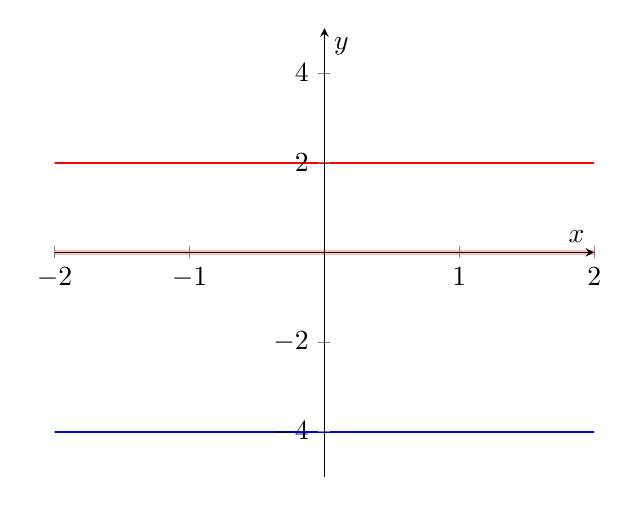
\begin{tikzpicture}
\begin{axis} [
	xmin=-2, xmax=2,
	ymin=-5, ymax=5,
	xlabel=$x$,ylabel=$y$,
	axis lines=center,
	axis on top=true,
	]
	\addplot	[draw=red, thick] {2};
	\addplot	[draw=pink, ultra thick] {0};
	\addplot	[draw=blue, thick] {-4};
\end{axis}
\end{tikzpicture}
\\\\\\
\indent
For $a = 31.9$
\\\\
\indent
$
A = \begin{bmatrix}-6&28&21\\4&-15&-12\\-8&31.9&25\end{bmatrix}
$
\\\\
\indent
The characteristic polynomial =
$
(-6 - \lambda)(-15 - \lambda)(25 - \lambda) + (28\times-12\times-8) + (21\times4\times31.9) - 
$
\\
\indent\indent\indent\indent\indent\indent\indent\indent\indent\indent\space\space\space
$
(-8\times21)(-15-\lambda) - (31.9\times-12)(-6-\lambda) - (4\times28)(25-\lambda)
$
\\\\
\indent\indent\indent\indent\indent\indent\indent\indent\indent\space\space\space\space
$
= -\lambda^3 + 4\lambda^2 + 435\lambda + 2250 + 2688 + 2679.6 - 2520 - 168\lambda - 2296.8 - 382.8\lambda - 
$
\\
\indent\indent\indent\indent\indent\indent\indent\indent\indent\indent\space\space\space
$
2800 + 112\lambda
$
\\\\
\indent\indent\indent\indent\indent\indent\indent\indent\indent\space\space\space\space
$
= -\lambda^3 +4\lambda^2 - 3.8\lambda + .8
$
\\\\
\indent
The eigenvalues are 1, 2.70416, and 0.295841.
\\\\
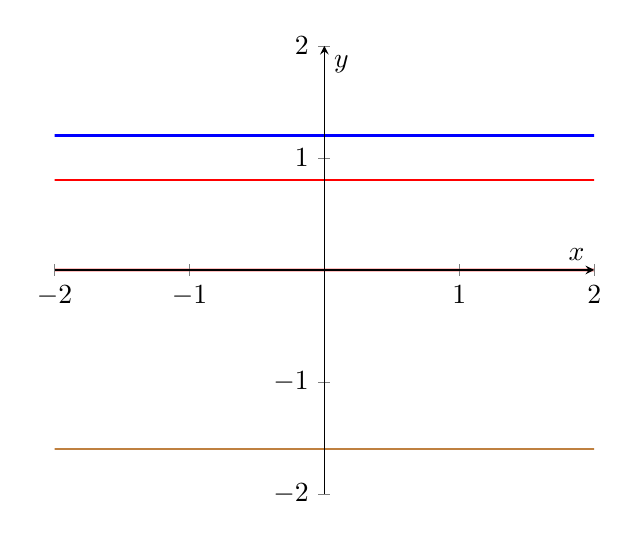
\begin{tikzpicture}
\begin{axis} [
	xmin=-2, xmax=2,
	ymin=-2, ymax=2,
	xlabel=$x$,ylabel=$y$,
	axis lines=center,
	axis on top=true,
	]
	\addplot	[draw=red, thick] {.8};
	\addplot	[draw=pink, ultra thick] {0};
	\addplot	[draw=blue, thick] {1.2};
	\addplot	[draw=brown, thick] {-1.6};
\end{axis}
\end{tikzpicture}
\\\\
\indent
For $a = 31.8$
\\\\
\indent
$
A = \begin{bmatrix}-6&28&21\\4&-15&-12\\-8&31.8&25\end{bmatrix}
$
\\\\
\indent
The characteristic polynomial =
$
(-6 - \lambda)(-15 - \lambda)(25 - \lambda) + (28\times-12\times-8) + (21\times4\times31.8) - 
$
\\
\indent\indent\indent\indent\indent\indent\indent\indent\indent\indent\space\space\space
$
(-8\times21)(-15-\lambda) - (31.8\times-12)(-6-\lambda) - (4\times28)(25-\lambda)
$
\\\\
\indent\indent\indent\indent\indent\indent\indent\indent\indent\space\space\space\space
$
= -\lambda^3 + 4\lambda^2 + 435\lambda + 2250 + 2688 + 2671.2 - 2520 - 168\lambda - 2289.6 - 381.6\lambda - 
$
\\
\indent\indent\indent\indent\indent\indent\indent\indent\indent\indent\space\space\space
$
2800 + 112\lambda
$
\\\\
\indent\indent\indent\indent\indent\indent\indent\indent\indent\space\space\space\space
$
= -\lambda^3 +4\lambda^2 - 2.6\lambda -0.4
$
\\\\
\indent
The eigenvalues are 1, -0.127882, and 3.12788.
\\\\
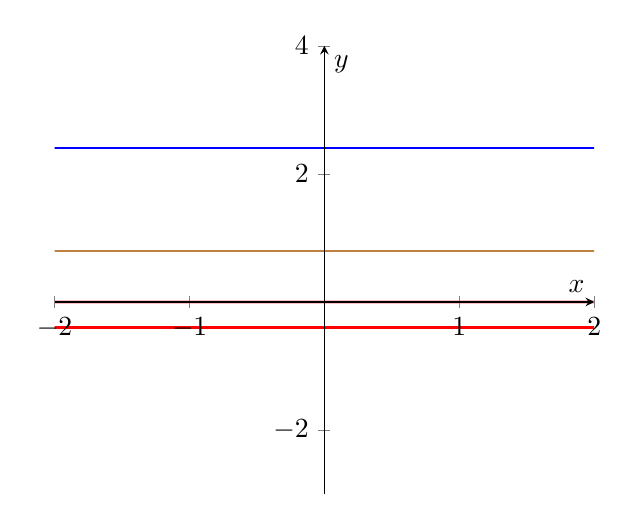
\begin{tikzpicture}
\begin{axis} [
	xmin=-2, xmax=2,
	ymin=-3, ymax=4,
	xlabel=$x$,ylabel=$y$,
	axis lines=center,
	axis on top=true,
	]
	\addplot	[draw=red, thick] {-.4};
	\addplot	[draw=pink, ultra thick] {0};
	\addplot	[draw=blue, thick] {2.4};
	\addplot	[draw=brown, thick] {.8};
\end{axis}
\end{tikzpicture}
\\\\\\
\indent
For $a = 32.1$
\\\\
\indent
$
A = \begin{bmatrix}-6&28&21\\4&-15&-12\\-8&32.1&25\end{bmatrix}
$
\\\\
\indent
The characteristic polynomial =
$
(-6 - \lambda)(-15 - \lambda)(25 - \lambda) + (28\times-12\times-8) + (21\times4\times32.1) - 
$
\\
\indent\indent\indent\indent\indent\indent\indent\indent\indent\indent\space\space\space
$
(-8\times21)(-15-\lambda) - (32.1\times-12)(-6-\lambda) - (4\times28)(25-\lambda)
$
\\\\
\indent\indent\indent\indent\indent\indent\indent\indent\indent\space\space\space\space
$
= -\lambda^3 + 4\lambda^2 + 435\lambda + 2250 + 2688 + 2696.4 - 2520 - 168\lambda - 2311.2 - 385.2\lambda - 
$
\\
\indent\indent\indent\indent\indent\indent\indent\indent\indent\indent\space\space\space
$
2800 + 112\lambda
$
\\\\
\indent\indent\indent\indent\indent\indent\indent\indent\indent\space\space\space\space
$
= -\lambda^3 +4\lambda^2 - 6.2\lambda + 3.2
$
\\\\
\indent
The eigenvalues is 1.
\\\\
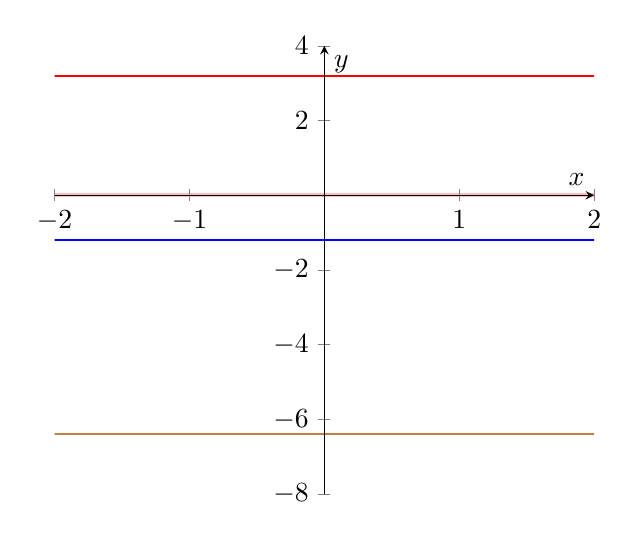
\begin{tikzpicture}
\begin{axis} [
	xmin=-2, xmax=2,
	ymin=-8, ymax=4,
	xlabel=$x$,ylabel=$y$,
	axis lines=center,
	axis on top=true,
	]
	\addplot	[draw=red, thick] {3.2};
	\addplot	[draw=pink, ultra thick] {0};
	\addplot	[draw=blue, thick] {-1.2};
	\addplot	[draw=brown, thick] {-6.4};
\end{axis}
\end{tikzpicture}
\\\\\\
\indent
For $a = 32.2$
\\\\
\indent
$
A = \begin{bmatrix}-6&28&21\\4&-15&-12\\-8&32.2&25\end{bmatrix}
$
\\\\
\indent
The characteristic polynomial =
$
(-6 - \lambda)(-15 - \lambda)(25 - \lambda) + (28\times-12\times-8) + (21\times4\times32.2) - 
$
\\
\indent\indent\indent\indent\indent\indent\indent\indent\indent\indent\space\space\space
$
(-8\times21)(-15-\lambda) - (32.2\times-12)(-6-\lambda) - (4\times28)(25-\lambda)
$
\\\\
\indent\indent\indent\indent\indent\indent\indent\indent\indent\space\space\space\space
$
= -\lambda^3 + 4\lambda^2 + 435\lambda + 2250 + 2688 + 2704.8 - 2520 - 168\lambda - 2318.4 - 386.4\lambda - 
$
\\
\indent\indent\indent\indent\indent\indent\indent\indent\indent\indent\space\space\space
$
2800 + 112\lambda
$
\\\\
\indent\indent\indent\indent\indent\indent\indent\indent\indent\space\space\space\space
$
= -\lambda^3 +4\lambda^2 - 7.4\lambda + 4.4
$
\\\\
\indent
The eigenvalues is 1.
\\\\
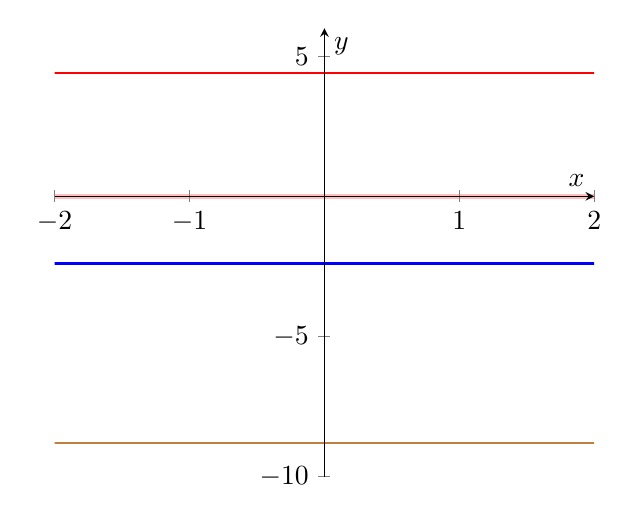
\begin{tikzpicture}
\begin{axis} [
	xmin=-2, xmax=2,
	ymin=-10, ymax=6,
	xlabel=$x$,ylabel=$y$,
	axis lines=center,
	axis on top=true,
	]
	\addplot	[draw=red, thick] {4.4};
	\addplot	[draw=pink, ultra thick] {0};
	\addplot	[draw=blue, thick] {-2.4};
	\addplot	[draw=brown, thick] {-8.8};
\end{axis}
\end{tikzpicture}
\\\\
\noindent\textbf{Question 3}
\\\\\
\indent
$
T(3b_1 - 4b_2) = \begin{bmatrix}0&-6&1\\0&5&-1\\1&-2&7\end{bmatrix}\begin{bmatrix}3\\-4\\0\end{bmatrix} =\begin{bmatrix}24\\-20\\11\end{bmatrix}
$
\\\\
\noindent\textbf{Question 4}
\\\\
\indent(a)
$
= \begin{bmatrix}5 + 3(-1)\\5 + 3(0)\\5+ 3(1)\end{bmatrix} = \begin{bmatrix}2\\5\\8\end{bmatrix}
$
\\\\
\indent(b)
\\\\
\indent\indent
Let
$
m = ax^2 + bx + c
$
and
$
n = dx^2 + ex + f
$
\\\\
\indent\indent
$
T(m + n) = T((a+d)x^2 + (b+e)x + c + f) = \begin{bmatrix}(a+d) - (b+e) + c + f\\c + f\\(a + d) + (b + e) + c + f\end{bmatrix} = \begin{bmatrix}a - b + c\\c\\a + b + c\end{bmatrix} + \begin{bmatrix}d - e + f\\f\\d + e + f\end{bmatrix} 
$
\\
\indent\indent\indent\indent\space\space\space\space
$
= T(m) + T(n)
$
\\\\
\indent\indent\indent
So $T(a + b) = T(a) + T(a)$
\\\\
\indent\indent
Let
$
m = ax^2 + bx + c
$
and $d$ is a scalar
\\\\
\indent\indent
$
T(dm) = \begin{bmatrix}da - db + dc\\dc\\da + db + c\end{bmatrix} = d\begin{bmatrix}a - b + c\\c\\a + b + c\end{bmatrix} = dT(m)
$
\\\\
\indent\indent\indent
So $T(ca) = cT(a)$
\\\\
\indent\indent
As $T(a + b) = T(a) + T(a)$ and $T(ca) = cT(a)$, T is a linear transformation.
\\\\
\indent(c)
\\\\
\indent\indent
$T$ relative to the basis $\{1, t, t^2\}$
\\\\
\indent\indent
Let $m = ax^2 + bx + c$
\indent\indent
$
T\times\begin{bmatrix}c\\b\\a\end{bmatrix} = \begin{bmatrix}a - b + c\\c\\a + b + c\end{bmatrix}
$
\indent\indent
$
T = \begin{bmatrix}1&0&1\\1&0&0\\1&1&1\end{bmatrix}
$
\\\\
\indent\indent
$T$ relative to the standard basis
\\\\
\indent\indent
Let $m = \begin{bmatrix}c\\b\\a\end{bmatrix}_{IP^2}$
\indent\indent
$
T \times \begin{bmatrix}c\\bt\\at^2\end{bmatrix} = \begin{bmatrix}a - b + c\\c\\a + b + c\end{bmatrix}
$
\indent\indent
$
T = \begin{bmatrix}1&-1/t&1/t^2\\1&0&0\\1&1/t&1/t^2\end{bmatrix}
$
\\\\
\noindent\textbf{Question 5}
\\\\
\indent(a) Find the eigenvalues of A
\\\\
\indent\indent
$
(-\lambda)(4-\lambda) - (-3 \times 1) = 0
$
\indent
$
-4\lambda+\lambda^2 + 3 = 0
$
\indent
$
(\lambda-1)(\lambda-3) = 0
$
\indent
$
\lambda = 1, 3
$
\\\\
\indent\indent
According to the theorem, if $A = PDP^{-1}$, the column of $P$ is the basis of $\beta$ and $D$ is $T_\beta$.
\\\\
\indent\indent
Find $P$
\\\\
\indent\indent
$\lambda = 1$
\indent\indent\indent\indent\indent\indent\indent\indent\indent\indent\indent\indent\indent
$\lambda = 3$
\\\\
\indent\indent
$
\begin{bmatrix}-1&1\\-3&3\end{bmatrix}x = 0
$
\indent
$
x = span\{\begin{bmatrix}1\\1\end{bmatrix}\}
$
\indent\indent\indent\indent\space\space\space
$
\begin{bmatrix}-3&1\\-3&1\end{bmatrix}x = 0
$
\indent
$
x = span\{\begin{bmatrix}-1/3\\1\end{bmatrix}\}
$
\\\\\\
\indent\indent
So $P = \begin{bmatrix}1&-1/3\\1&1\end{bmatrix}$ and $D = \begin{bmatrix}1&0\\0&3\end{bmatrix}$. The basis $\beta$ is $\{\begin{bmatrix}1\\1\end{bmatrix}, \begin{bmatrix}-1/3\\1\end{bmatrix}\}$
\\\\
\indent(b) Follow the same procedure as part (a)
\\\\
\indent\indent
$
(5-\lambda)(1-\lambda) - (-7\times-3) = 0
$
\indent
$
5-6\lambda+\lambda^2-21 = 0
$
\indent
$
\lambda = -2, 8
$
\\\\
\indent\indent
Find $P$
\\\\
\indent\indent
$\lambda = -2$
\indent\indent\indent\indent\indent\indent\indent\indent\indent\indent\indent\indent\indent
$\lambda = 8$
\\\\
\indent\indent
$
\begin{bmatrix}7&-3\\-7&3\end{bmatrix}x = 0
$
\indent
$
x = span\{\begin{bmatrix}3/7\\1\end{bmatrix}\}
$
\indent\indent\indent\indent
$
\begin{bmatrix}-3&-3\\-7&-7\end{bmatrix}x = 0
$
\indent
$
x = span\{\begin{bmatrix}-1\\1\end{bmatrix}\}
$
\\\\\\
\indent\indent
So the basis $\beta$ is $\{\begin{bmatrix}3/7\\1\end{bmatrix}, \begin{bmatrix}-1\\1\end{bmatrix}\}$
\\\\
\noindent\textbf{Question 6}
\\\\
\indent(a) Find the covariance matrix.
\\\\
\indent(b) Find the covariance matrix of the matrix \textit{img\_in}. It is required since eig() function requires the input to be a square matrix. cov() convert a rectangular matrix into a square matrix. The value of each cell indicates the distance of data from the average.
\\\\
\indent(c) Find the eigenvalues and eigenvectors.
\\\\
\indent(d) V is a matrix whose columns are eigenvectors and D is a diagonal matrix of the corresponding eigenvalues.
\\\\
\indent(e)
$V^{-1} = V^T$
$\longrightarrow$
$V^{-1} \times V = V^T \times V$
$\longrightarrow$
$I = V^T \times V$
\\
\indent\indent
Because $A = cov$(\textit{img\_in}) is a symmetric matrix, A can be decomposed as $PDP^{-1}$ where P is an orthogonal matrix. In this case, $V$ is the same as $P$. As the property of a orthogonal matrix, $P\times P^{T} = P^{T}\times P = I$. As a result, the given equation is true.
\\\\
\indent(f) The code change the basis from the standard basis to the the basis of the largest 110 eigenvectors and the image get compressed.
\\\\
\indent(g) 530 to 640 indicates that the \textit{img\_in} was compressed by the largest 110 eigenvectors. They are sufficient because they can span most data of the image. The image loses some detail, but the important detail is still preserved.
\\\\
\indent(h) A image with vertical blue lines. The image loses its important detail because the smallest 400 eigenvectors are much far away from the mean of the data, so they contains unnecessary data.
\\\\
\indent(i) It changes the basis of \textit{img\_in} from the standard basis to the largest 110 eigenvecttors.
\end{document}